\documentclass{bioinfo}
\copyrightyear{2013}
\pubyear{2013}

\newcommand{\Espresso}{Espresso}

\newcommand{\kmer}{$k$-mer{}}
\newcommand{\kmers}{$k$-mers{}}
\newcommand{\dna}[1]{\hbox{\small \texttt{\uppercase{#1}}}}

\newtheorem{defn}{Definition}

\usepackage{multirow}
\begin{document}
\firstpage{1}

\author{
Thomas Conway \\
Andrew Bromage \\
Jeremy Wazny
}

\title[\Espresso{}]{Espresso: Fast Gene Expression Analysis of RNA-seq data}
\author[Conway \textit{et~al}]{Thomas Conway\footnote{to whom correspondence sho
uld be addressed}\ , Andrew Bromage and Jeremy Wazny}
\address{NICTA Victoria Research Laboratory, Department of Computer Science and 
Software Engineering, The University of Melbourne, Parkville, Australia\\
}

\history{Received on XXXXX; revised on XXXXX; accepted on XXXXX}

\editor{Associate Editor: XXXXXXX}

\maketitle

\begin{abstract}

\section{Motivation:}
RNA-seq is a rapidly growing technique for biological investigation.
Popular analysis tools based on read alignment produce a wealth of
information which is often left unused by investigators, who often
want simple measures of (differential) gene expression. These tools
provide this information, but are often expensive to run.

\section{Results:}
Using \kmer\ based techniques, we have developed an alignment-free
method for computing relative gene expression, using a principled
statistical model for assigning reads to transcripts.
We find that this method is both fast and accurate.

\section{Availability:}
\Espresso{} is available for non-commercial use 
from http://www.genomics.csse.unimelb.edu.au/product-espresso.php.

\section{Contact:} \href{tom.conway@nicta.com.au}{tom.conway@nicta.com.au}
\end{abstract}

\section{Introduction}
\label{sec:intro}

The available of low cost high throughput sequencing is making
RNA-seq an increasingly attractive tool for biological investigation
into gene expression and other transcriptionally mediated processes.
RNA-seq is an attractive tool for investigating transcripts
because it can provide very detailed information: relative abundance,
alternate splicing, post-transcriptional editing, SNVs, and so on.

The volume of data involved in RNA-seq experiments is enormous, and
often overwhelming for investigators.
It is often the case that when analysis is performed, the vast majority
of the analysis products are ignored as the investigators quickly
narrow in on specific genes.
Moreover, even where the genome of an organism is conserved across
individuals, transcription has high variability across tissues and
conditions.

Existing methods for computing relative gene expression, typically
measured in units of fragments per kilobase of transcript per million
mapped reads, or FPKM~\citep[see][]{Trapnell:2010}, are
generally alignment-based.
Reads are aligned to a reference genome or a set of reference
transcripts (or to inferred contigs, in the case of \textit{de~novo}
transcriptome assembly) and the alignments are analyzed.  This
analysis may be as simple as counting the number of fragments (reads,
or read pairs) associated with a previously annotated gene; it may
include the inference of novel transcripts, such as unannotated
genes or unannotated splice variants; resolution of allele specific
expression; and it may include detailed analysis to resolve the
relative abundance among alternate isoforms of
genes~\citep[e.g.][]{Jiang:2009,Li:2010}.

Even before this analysis is done, alignments must be performed.
When carried out against a reference genome, splice junctions present
a significant obstacle to simple alignment~\citep{Pepke:2009}.
The resulting algorithms to compensate tend to be substantially more
expensive than regular alignment.
Alignment to a set of reference transcripts is both conceptually
and computationally simpler, but can still be problematic.
If the sample contains novel transcripts,
these may be lost in the analysis, or at least yield confusing
results~\citep{Marioni:2008}.

Performing detailed (and usually expensive) analysis which will be mostly
unused is both time consuming and wasteful of computational resources.
We believe an analysis tool that allows an investigator to quickly associate
reads with transcripts is a practical way to make RNA-seq analysis more
efficient.
The goal is not to supplant existing alignment-based methods, but rather
to allow investigators to use the existing methods in more targeted ways,
on relevant subsets of their data.

In previous work~\citep{Xenome:2012} we observed that on mammalian genomes
(human and mouse, in particular), the high degree of genomic (and
transcriptomic) conservation means that \kmer{}, or
alignment-free~\citep{Vinga:2003}, techniques are very effective
as well as efficient.

There are two novel contributions in this paper:
first, we introduce a simple, yet principled statistical model for using reads
as evidence for transcript expression;
second, we introduce a representation of an inverted index
over \kmers\ using a sparse bit matrix, which supports an efficient
method for parameter learning using this model.

\section{Methods}

\subsection{Preliminaries}

\begin{defn}[\kmer{} canonicalization]

Consider a \kmer~$x$. We denote its reverse complement by $\bar{x}$.

A \textit{canonical \kmer{}}~$\hat{x}$ is defined by a choice function $\mathcal{C}$
giving a deterministic choice between $x$ and $\bar{x}$:
$$
    \forall x: \hat{x} = \mathcal{C}(x) = \mathcal{C}(\bar{x})
$$
That is, for all \kmers\ a consistent,
but arbitrary choice is made between a \kmer\ and its reverse complement.
Example choice functions include choosing the lexicographically smaller of $x$ and $\bar{x}$,
or choosing the one with a smaller hash value.
\end{defn}

\begin{defn}[substrings of sequences]
Consider a nucleotide sequence $s$.
We write the length of $s$ as $|s|$.
The individual nucleotides may be addressed $s[0], s[1], \ldots, s[|s| - 1]$.

Substrings of $s$ are written using a half-open interval semantics, with $s[b,e]$
refering to the substring composed of the nucleotides $s[b], s[b+1], \ldots, s[e - 1]$.
\end{defn}

\begin{defn}[$k$-merization of sequences]
For a given nucleotide sequence $s$, we define the function $\mathcal{K}_k(s)$ which is the set of
canonical \kmers\ which may be derived from $s$.

More formally:
$$
\mathcal{K}_k(s) = \{\mathcal{C}\left(s[i, i + k]\right) : 0 \le i < |s| - k + 1 \}
$$

Note that
$$
	\forall s: \mathcal{K}_k(s) = \mathcal{K}_k(\bar{s})
$$
That is, the set of canonical \kmers\ in a sequence $s$ is the same as the set of canonical
\kmers\ in its reverse complement.
\end{defn}

\begin{figure}
\begin{center}
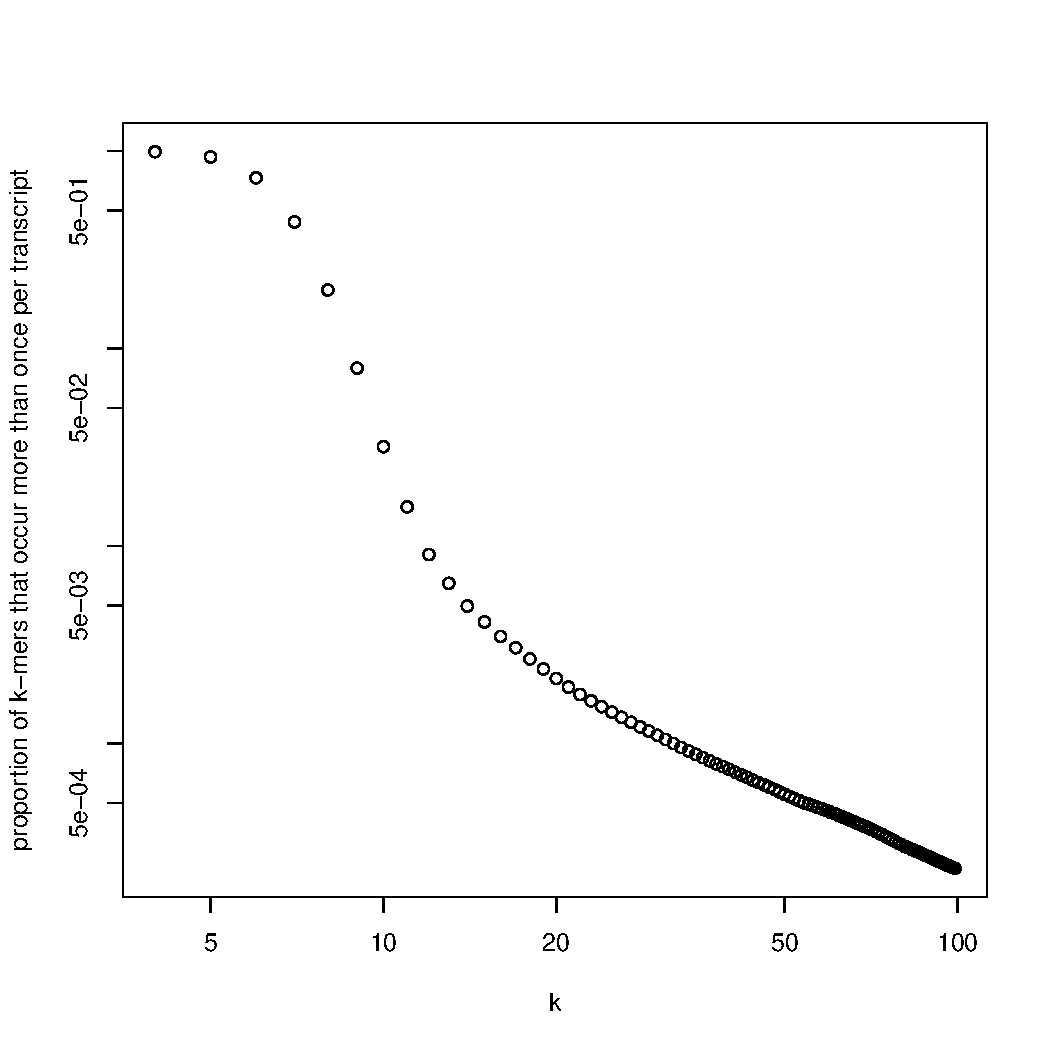
\includegraphics[scale=0.45]{{data/kmer-uniqueness}.pdf}
\end{center}
\caption{
A plot showing the proportion of \kmers\ that are unique within a transcript for
various values of $k$. Note the log-log scale.
}
\label{fig:uniqueness}
\end{figure}

For a given transcript sequence $g$, with length $|g|$ the set of \kmers\ in that transcript is $\mathcal{K}_k(g)$.
If there are no duplicated \kmers\ (which is approximately true for $k > 15$, see Figure~\ref{fig:uniqueness}),
then $|g| \approx |\mathcal{K}_k(g)|$.

\begin{defn}[sequence reads]
A \textit{sequence read}, or simply a \textit{read} is an exprimentally
derived substring of a transcript.  That is, for a given transcript $g$, a read
$r$ is a length $L$ substring of $g$, or its reverse complement.
(Note that because we shall be considering only the sets of canonical
\kmers\ that are derived from reads, we can henceforth ignore reverse
complement reads.) Therefore, the set of reads that may be derived
from a transcript is
$$
	\{g[i, i + L] : 0 \le i < |g| - L + 1 \} \cup \{\bar{g}[i, i + L]: 0 \le i < |g| - L + 1 \}
$$

\end{defn}

\subsection{A Bayesian Model}
\label{sec:bayes}

Using a collection of reads as evidence, we wish to estimate the relative expression of
each transcript out of a collection of transcripts.
We may interpret a vector $\mathbf{g}$ representing the relative expression of each
transcript in the collection as representing the relative probability that a
read derived from the sample will arise from a given transcript.

\begin{figure}
\begin{center}
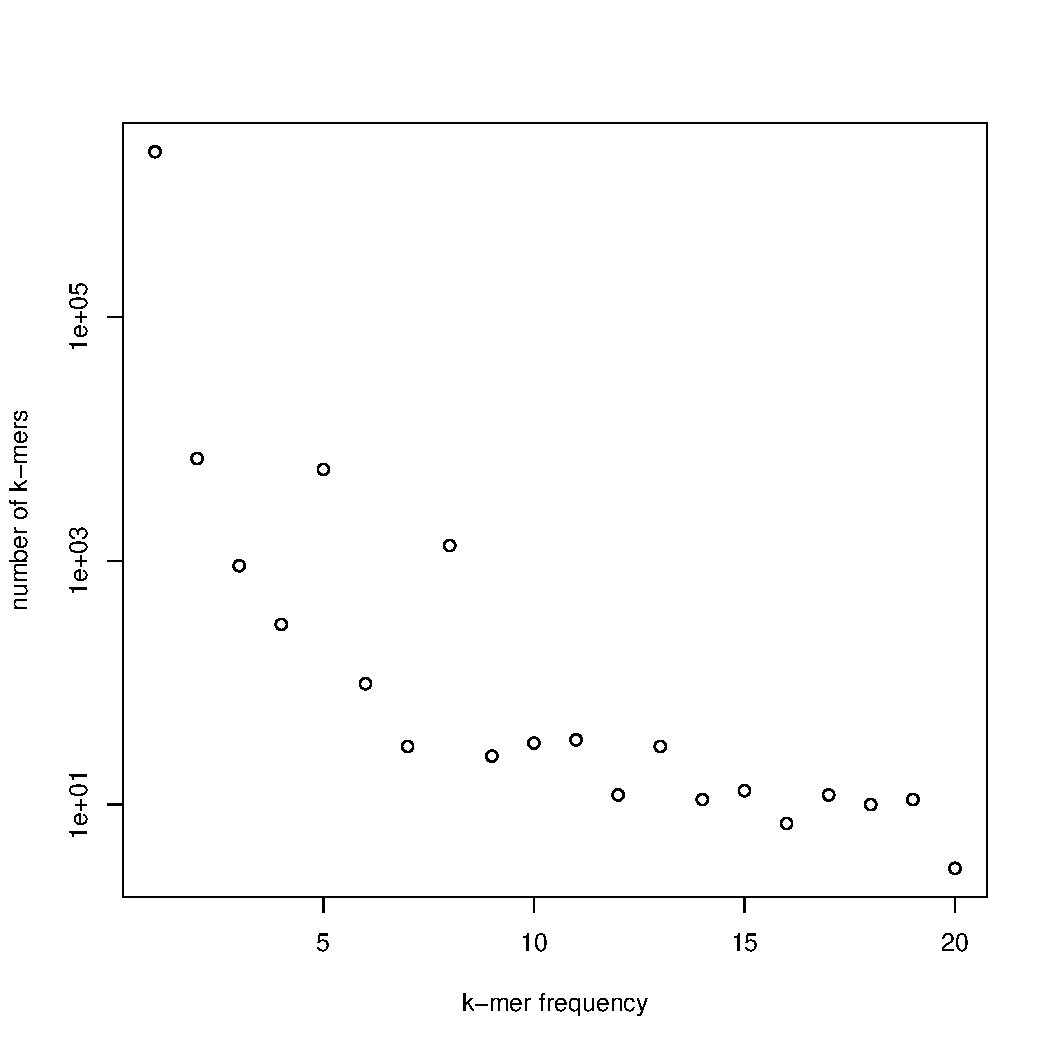
\includegraphics[scale=0.45]{{data/staph-kmer-frequencies}.pdf}
\end{center}
\caption{
Histogram showing the number of transcripts that 20-mers occur in
across the set of 2,734 genes in Staphylococcus aureus (strain N315).
}
\label{fig:staphkmers}
\end{figure}

\begin{figure}
\begin{center}
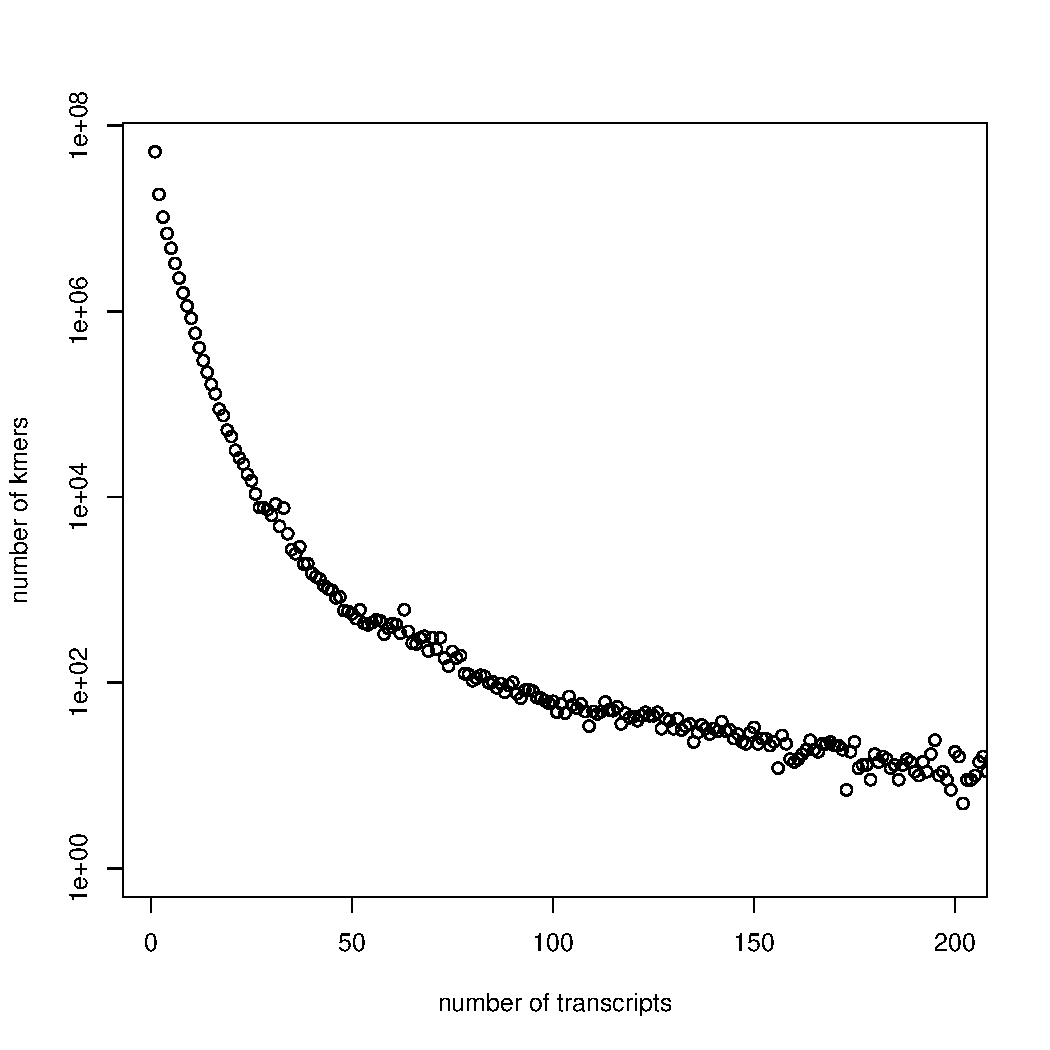
\includegraphics[scale=0.45]{{data/kmer-hist}.pdf}
\end{center}
\caption{
Histogram showing the number of transcripts that 25-mers occur in
across the set of 180,107 gencode~V12 transcripts.  For example,
the left most point shows that almost $10^8$ 25-mers occur in only
one transcript.  The tail of the histogram is long but low --- the
extremum is a single 25-mer occuring in 5,976 transcripts.
}
\label{fig:kmers}
\end{figure}

In the set of reference transcripts for a simple organism such as Staphylococcus aureus (strain N315),
the overwhelming majority of 20-mers (97\%) occur in a single gene, so in most
cases, even allowing for the fact that some genes have significant homology,
and that genes are not composed of arbitrary
\kmers\ but related sets, reads can be attributed unambiguously to genes.

In more complex organisms it is typically the case that there is a significantly more complex transcriptional
landscape including near homologues, splice variants and non-coding RNAs. In the Gencode human transcriptome,
only 19\% of 25-mers are unique to a single transcript.
Therefore, a more subtle approach is needed. Our approach revolves around computing a probability that the
set of \kmers\ in a read arose from each transcript, and combining that probability with a prior assumption about
the relative abundance of that transcript, and using that to update the priors for the processing of the next read.

As such, we adopt a Bayesian model using a multinomial distribution with a Dirichlet
prior.
\begin{equation}\label{eqn:gr}
	\textrm{Pr}(\mathbf{g}|r) =
		\frac{\textrm{Pr}(r|\mathbf{g}) \textrm{Pr}(\mathbf{g})}{\textrm{Pr}(r)}
\end{equation}

The posterior probability $\textrm{Pr}(\mathbf{g}|r)$ after seeing each read is used
to update the prior $\textrm{Pr}(\mathbf{g})$ for the next read. This yields an on-line
algorithm for estimating the true posterior probabilities over a collection of reads $\mathbf{R}$:
$\textrm{Pr}(\mathbf{g}|\mathbf{R})$.
This is a similar model to that used by CuffExpress~\citep{Roberts:2011}.

The core of this algorithm is the computation of the likelihood of observing a particular read
from a given transcript $\textrm{Pr}(r|g)$. We compute this using \kmer\ decompositions of
transcripts and reads. This probability is calculated for each read across all transcripts,
and normalized to yield $\textrm{Pr}(r|\mathbf{g})$.

Consider a read $r$. If $r$ is drawn from $g$, then it must be one
of $|g| - |r| + 1$ possibilites.
Consequently there are approximately
$|\mathcal{K}_k(g)|$ possible sets of $k$-mers that may be observed
from read drawn from $g$, assuming $|g| \gg |r|$ and no errors or SNVs,
and we can therefore write the probability of observing a read arising from a particular position:
\begin{equation}\label{eqn:r}
\textrm{Pr}_{\textit{pos}}(r|g) \approx \frac{1}{|g| - |r| + 1}
\end{equation}

If a read $r$ containing possible divergences (i.e. errors and SNVs)
arises from a transcript $g$, we expect most $k$-mers to exist in
the intersection, with some missing due to sequence variation and
sequencing error.

The number of missing \kmers\ that are in $r$ but not in the intersection of $r$ and $g$ is
$$
M_{g,r} = \left| \mathcal{K}_k(r) - \left(\mathcal{K}_k(g) \cap \mathcal{K}_k(r) \right) \right|
$$

If we wish to estimate the number of divergent bases
(assuming substitutions, not indels, which is a reasonable assumption for
the most common sequencing platforms) in a read, we make the observation that
a single substitution will alter up to $k$ \kmers.
If the substitution occurs in the middle of the read it will alter
all $k$ \kmers\ that cross it. If it occurs near the beginning
or end of the read, it will alter fewer \kmers.
For values of $k$ where most \kmers\ are unique,
the probability of an altered \kmer\ from a read occurring in the gene is very low.
This leads us to estimate $E_{g,r}$,the number of divergences, as
$$
\lceil M_{g,r} / k \rceil \le E_{g,r} \le M_{g,r}
$$

In practice, we use the upper bound for three reasons.
Firstly, sequencing errors tend to be biased towards the ends of reads.
Secondly, transcribed sequences (especially protein coding sequences)
tend to be fairly highly conserved, so contain relatively few SNVs.
Finally, when evaluating $\textrm{Pr}(r|g)$ for a read which genuinely
comes from a different transcript, the lower bound tends to under-estimate
the number of errors.

If we assume a divergence rate of $e$ (typically around $0.01$),
we can express the probability of observing values of $E_{g,r}$ in terms of binomial
probability, and can express the probability of observing a particular number of errors:
\begin{equation}\label{eqn:e}
\textrm{Pr}_{\textit{errors}}(r|g) \approx \textrm{Bin}(e, |r|, X \ge E_{g,r}) \cdot
	\frac{1}{\textrm{F}(e, |r|)}
\end{equation}
Where
Where $\textrm{F}(e, |r|)$ is a normalization term
$$
	\textrm{F}(p, n) = \sum\limits_{i=0}^{n} \textrm{Bin}(p, n, X \ge i)
$$
Since~$F$ depends only on read length and divergence rate, it is the same across all genes,
and its omission may be compensated for in subsequent normalization,
so we can drop it from the computation of $\textrm{Pr}(r|g)$ in practice.


Composing Equation~\ref{eqn:r} and Equation~\ref{eqn:e},
we have the following espression of the probability of a
read being observed arising from a given gene:
\begin{equation}\label{eqn:rg}
\textrm{Pr}(r|g) \approx \frac{\textrm{Bin}(e, |r|, X \ge E_{g,r})}{|g| - |r| + 1} \cdot
	\frac{1}{\textrm{F}(e, |r|)}
\end{equation}

\subsection{Implementation Concerns}\label{sect:implementation}

Our goal is to make the computation of relative gene expression efficient,
so some attention to implementation details is important.
The method is efficient in two senses. On the one hand, we use a space-efficient
representation of the reference transcripts, and on the other, the use of \kmer\ based
matching rather than doing full alignment is time-efficient.

\begin{figure}
\begin{center}
\includegraphics[scale=0.7]{pict-matrix.pdf}
\end{center}
\caption{An outline of the data structure described in
Section~\ref{sect:implementation}.
The set of all \kmers\ found in the reference transcripts is implemented
using a sparse bitmap.
The sets of \kmers\ found in the individual reference transcripts may
then be represented using a binary matrix.
In this example, there are only~8 \kmers\ in the entire set of reference
transcripts.
The rank of each extant \kmer\ in the sparse bitmap provides the column index
for the matrix $A$.
For example, the \kmer\ \dna{cgac} has rank~4, which represents column~4
in $A$ (assuming that the matrix is zero-indexed).
In this column, entries~$A_{04}$ and~$A_{24}$ are $1$, indicating that
transcripts~0 and~2, but not~1, contain the \kmer\ \dna{cgac}.
}
\label{fig:matrix}
\end{figure}

The reference transcripts are decomposed into sets of canonical \kmers, the union
of which is stored in a single sparse bitmap using the techniques developed in our
previous work~\citep{Conway:2011p17913}.
This is used to implement a function which maps a \kmer\ $x$ to a
rank $v$ within the universe of \kmers\ that exist in the reference collection.

The individual set for each transcript is mapped with this function from being a
set over \kmers\ to a set over ranks. These sets are then compiled into a bit matrix
arranged so that for each rank,
a contiguous sequence of bits identifies the set of transcipts containing
the \kmer\ having that rank. (See Figure~\ref{fig:matrix}.)
This matrix is stored using a sparse bitmap also, and is accessed efficiently using
the \textit{rank/select} API as discussed in our previous work, cited above.
This matrix is large, but extremely sparse: with $k=25$, the set of 180,107 gencode~V12 transcripts,
contains a little over 104~million distinct \kmers. Figure~\ref{fig:kmers} shows
a histogram of \kmer\ frequencies. About half the \kmers\ occur in
only 1 transcript, and about 90\% of \kmers\ occur in~5 or fewer transcripts. That is,
half the columns in the matrix contain only one set bit, and~90\% contain~5 or fewer,
out of 180~thousand.

Traditional inverted index representations typically have a dictionary data structure
(e.g. search tree, hash table) to map from the domain of keys (i.e. \kmers{}) to \textit{postings vectors}
(i.e. lists of transcript identifiers).
\citet{ZobelMoffat:2006} give an overview of techniques used to implement these data structures.

Our representation is superficially similar, in that it has a sparse bitmap representing
the set of keys and a bit matrix representing the postings vectors.
The important difference is that the use of a sparse bitmap with \textit{rank}/\textit{select}
is that it transforms the sparse domain of \kmers\ into the dense domain of ranks, and it does
so in a very space efficient manner.
The representation of the postings as a sparse matrix in turn frees us from an ad-hoc
choice of postings layout/coding, and devolves the problem to the well studied one of
sparse bitmap representations which are close to optimal.

To process a read (or read pair), the read is decomposed into \kmers\ and each \kmer\ is
looked up in the sparse bitmap. Any \kmers\ that are not present in any transcript are ignored.
We compile a mapping that for each transcript gives the number of \kmers\ that were present in the read. For each transcript for which there is at least one \kmer\ conincident with the read,
we compute $\textrm{Pr}(r|g)$ according to Equation~\ref{eqn:rg}, and
the prior probabilities are incorporated according to Equation~\ref{eqn:gr}.
These quantities are then normalized so they sum to 1, and used to update the Dirichlet prior
for the next read.

\section{Results}

\begin{table}
\begin{center}
\begin{tabular}{|r|r|}
\hline
\textbf{Tool}    & \textbf{Running Time (m)} \\
\hline
Espresso         &   4 \\
Tophat/Cufflinks & 114 \\
RSEM             & 325 \\
\hline
\end{tabular}
\end{center}
\caption{Running time for evaluation. All experiments were run on a machine with 8 2GHz Opteron cores and 32MB RAM.}
\label{tbl:time}
\end{table}

\begin{table*}
\begin{center}
\begin{tabular}{|r|r|r|r|}
\hline
\textbf{Tool}    & \textbf{No Divergence} & \textbf{e=0.01} & \textbf{m=0.001 \& e=0.005} \\
\hline
Espresso         &   0.998 & 0.997 & 0.998 \\
Tophat/Cufflinks &   0.423 & 0.424 & 0.424 \\
RSEM             &   0.692 & 0.692 & 0.691 \\
\hline
\end{tabular}
\end{center}
\caption{
The correlations between the true expression levels and the expression levels reported by
the tools for the different data sets.
}
\label{tbl:cor}
\end{table*}

\begin{table*}
\begin{center}
\begin{tabular}{|r|r|r|r|r|r|r|}
\hline
\textbf{Data Set} & \textbf{Tool}    & $x < 10^0$ & $10^0 \le x < 10^1$ & $10^1 \le x < 10^2$ & $10^2 \le x < 10^3$ & $10^3 \le x$ \\
\hline
\multirow{3}{*}{No Divergence} & Espresso         &   3 & 0 & 2 & 1 & 0 \\
                                 & Tophat/Cufflinks &   32 & 5 & 3 & 0 & 2 \\
                                 & RSEM             &   0 & 3 & 1 & 0 & 0 \\
\hline
\multirow{3}{*}{e=0.01}          & Espresso         &   0 & 0 & 0 & 0 & 0 \\
                                 & Tophat/Cufflinks &   0 & 0 & 0 & 0 & 0 \\
                                 & RSEM             &   26 & 5 & 3 & 0 & 0 \\
\hline
\multirow{3}{*}{m=0.001 \& e=0.005}
			         & Espresso         &   24 & 10 & 4 & 1 & 0 \\
                                 & Tophat/Cufflinks &   37 & 4 & 3 & 2 & 0 \\
                                 & RSEM             &   13 & 1 & 2 & 0 & 0 \\
\hline
\end{tabular}
\end{center}
\caption{
The number of transcripts spuriously reported as expressed at different expression levels
for the tool/data set combinations.
}
\label{tbl:xtalk}
\end{table*}

\begin{figure*}
\begin{center}
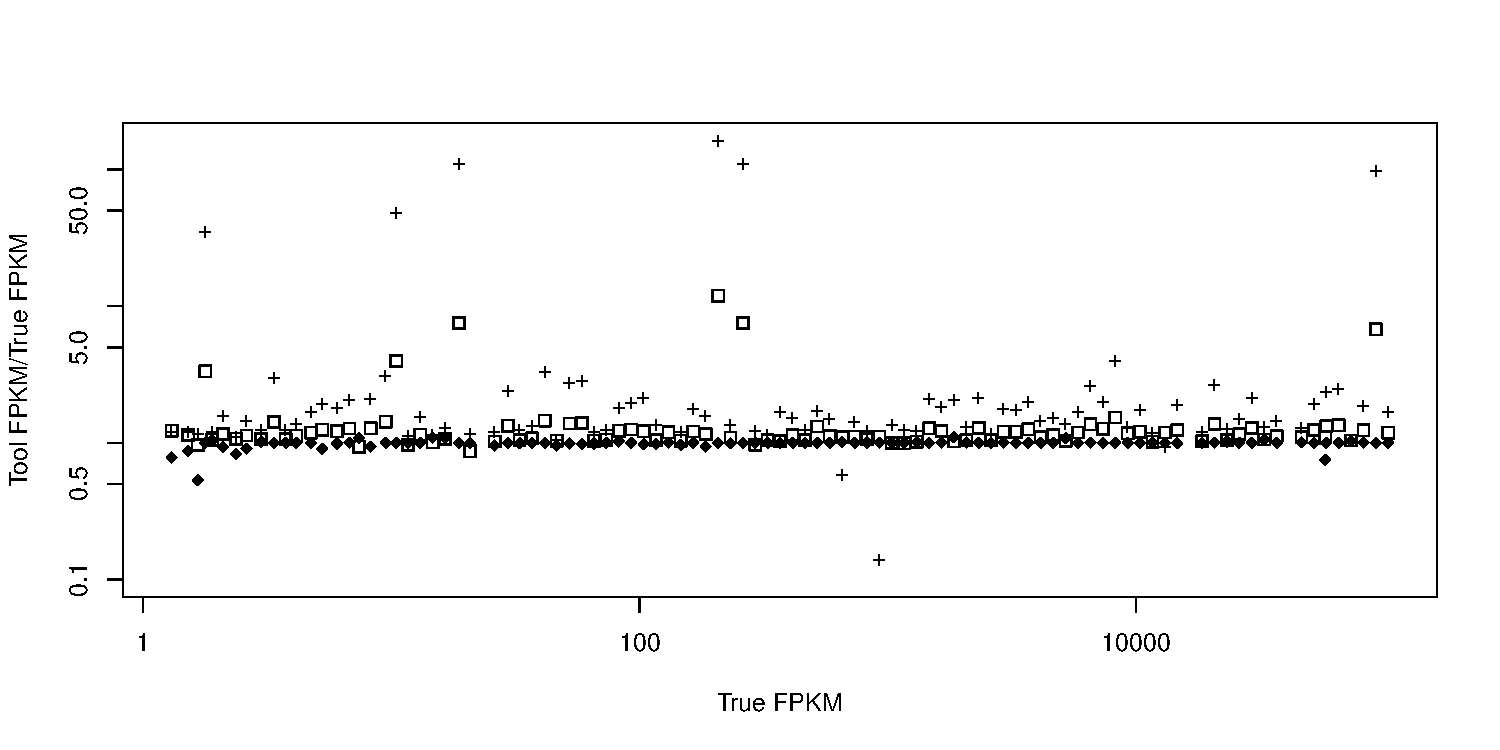
\includegraphics[scale=0.7]{{data/gen-fpkms}.pdf}
\end{center}
\caption{
The results of the experiment involving simulated RNA-seq data with no SNVs,
and no errors. The horizontal axis represents the true expression level, and the vertical axis the ratio between the expression level reported by the tools and the true expression level. A perfect tool would have all transcripts reported with a ratio of 1,
with a small level of noise due to sequencing error. The results of \Espresso{} are depicted with solid diamonds. The results to Tophat/Cufflinks are depicted with `+' symbols. The results of Bowtie + RSEM are reported with open squares.
}
\label{fig:fpkms0}
\end{figure*}

\begin{figure*}
\begin{center}
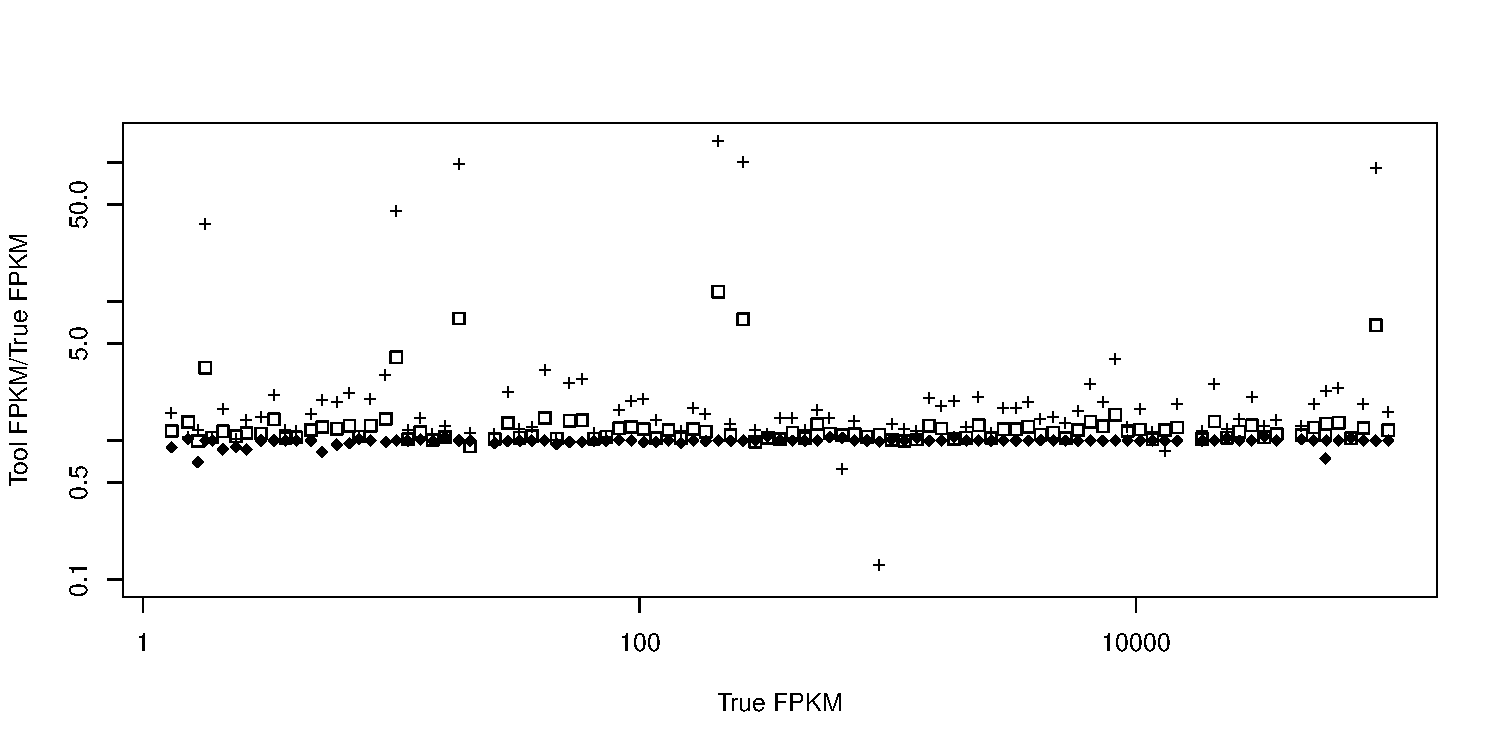
\includegraphics[scale=0.7]{{data/gen-e0.01-fpkms}.pdf}
\end{center}
\caption{
The results of the experiment involving simulated RNA-seq data with no SNVs,
and a substitution error rate of 1\% per base. The horizontal axis represents the true expression level, and the vertical axis the ratio between the expression level reported by the tools and the true expression level. A perfect tool would have all transcripts reported with a ratio of 1,
with a small level of noise due to sequencing error. The results of \Espresso{} are depicted with solid diamonds. The results to Tophat/Cufflinks are depicted with `+' symbols. The results of Bowtie + RSEM are reported with open squares.
}
\label{fig:fpkms1}
\end{figure*}

\begin{figure*}
\begin{center}
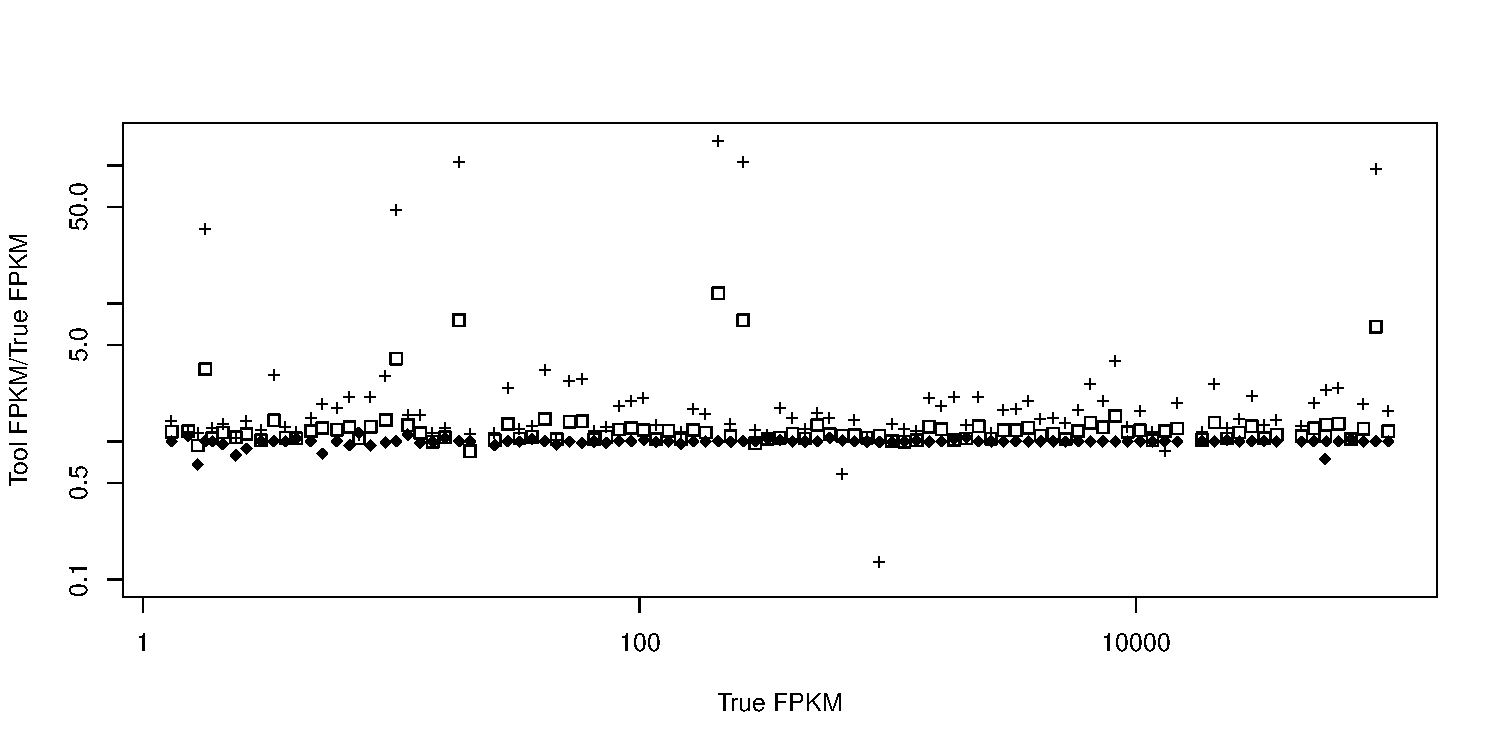
\includegraphics[scale=0.7]{{data/gen-m0.001-e0.005-fpkms}.pdf}
\end{center}
\caption{
The results of the experiment involving simulated RNA-seq data with a SNV rate of 0.1\% per base,
and a substitution error rate of 0.5\% per base. The horizontal axis represents the true expression level, and the vertical axis the ratio between the expression level reported by the tools and the true expression level. A perfect tool would have all transcripts reported with a ratio of 1,
with a small level of noise due to sequencing error. The results of \Espresso{} are depicted with solid diamonds. The results to Tophat/Cufflinks are depicted with `+' symbols. The results of Bowtie + RSEM are reported with open squares.
}
\label{fig:fpkms2}
\end{figure*}

The absence of a gold standard makes it difficult to evaluate the
accuracy of the method.  To overcome this, we have used simulated
data.  The reference data we have used is the Gencode v12 annotations,
with respect to GRCH37.  We have randomly selected 100 transcripts
from the reference set, and set an expression level for each chosen
from a range spanning 5 orders of magnitude devided into logarithmically
uniform divisions.  From this we have derived 3 sets each of just
over 8 million reads. The first set contains no simulated SNVs
and no errors. This is used to evaluate an expected best case
behaviour. The second set contains simulated errors at a uniform
rate of 1\% chance of a substitution in each base. This is used to
evaluate the tolerance of the method to noise. The third set contains
simulated SNVs at a rate of 0.1\% chance of a substitution at each
base and errors at a rate of 0.5\% chance of substitution per base.
This is used to evaluate the behaviour under systematic sequence
divergences and errors.

All experiments with \Espresso{} were performed using $k=25$.

The building of the \kmer\ set and other reference data structures took 19 minutes.
This need be done only once for a given set of reference transcripts.
The resulting reference data structures are 850MB in size.
For comparison, the corresponding bowtie index is 403MB.
Although the space is larger, it is still well within main memory scale on any
reasonable computer.

It is important to acknowledge that our model of introducing randomly
distributed SNVs probably leads to slightly optimistic results,
since especially in the case of coding transcripts, most real SNVs
are non-uniformly distributed.
However, we note that in the overwhelming majority of cases divergent
\kmers\ are simply absent from the set of reference \kmers\ and are
therefore ignored.

Since we know the expected FPKM for each transcript,
we can compare the results produced by \Espresso{} with the expected
value to establish the accuracy of our method. For comparison, we
have compared with two other tools: TopHat/Cufflinks~\citep{Trapnell:2010},
and RSEM~\citep{Li:2010}.

We would like to be able to compare with CuffExpress~\citep{Roberts:2011},
which uses a similar on-line algorithm to estimate transcript abundances,
but unfortunately, this tool is unavailable.

We have compared with Tophat/Cufflinks because it is widely used
for the purpose of producing lists of genes/transcripts with
associated FPKMs for downstream analysis, even though it computes
significantly more subtle and detailed information, including novel
transcripts, novel splice junctions, as well as the obvious products
such as SNP calling which result from performing alignments (which it does to a reference
\textit{genome}).

RSEM also performs alignments (though to a reference transcriptome), and
resolves ambiguous alignments to elucidate the abundance of individual isoforms.

All experiments were run on a single server with 8~Opteron cores and 32GB RAM.
The running times and memory usage are shown in Table~\ref{tbl:time}.

Figure~\ref{fig:fpkms0} shows the results for the first, error free, data set.
Figure~\ref{fig:fpkms1} shows the results for the second data set, with a 1\%
base substitution (error) rate.
Figure~\ref{fig:fpkms2} shows the results of the third data set with a 0.5\% base substitution
(error) rate, and a 0.1\% base SNV rate.

Table~\ref{tbl:cor} shows the correlation between the true expression
level and the experimentally determined expression level for each data set for each tool.

Table~\ref{tbl:xtalk} shows the number of transcripts with expression falsely attributed
to them, grouped according to the level of expression.

\section{Discussion}


The results presented above show that \Espresso{} is consistently able
to accurately assign coverage to transcripts.  There is a low level
of crosstalk in most cases.
The misassignment of coverage is potentially attributable to two
causes: errors/SNVs leading to \kmers\ which occur in a spurious
transcript; and strong homology between transcripts leading to
ambiguity.

The Spearman correlation between the results for the perfect reads and reads with errors
is~0.9999754 which suggests that errors are not contributing to crosstalk.
The correlation between the results for the perfect reads and the reads with 
errors and SNVs is~0.9999638, which suggests that the systematic divergences tend not
to contribute to crosstalk.

The most cases the crosstalk occurs between isoforms of the same
gene, or between homologous genes/pseudogenes.  There are certainly
pathological cases such as NCOR2 which has~25 recognised transcripts
in Ensembl,~7 of which are long and highly similar. Considering the
25-mers in NCOR2, there are over 8,500 which occur in at least~7
transcripts. In practice this means that most reads derived from
ones of these~7 transcripts will be completely ambiguous, and so
only a minority of \kmers\ will be distinctive to the truly expressed
transcript(s).  However most of the \kmers\ that arise from the
NCOR2 transcripts, don't occur in any other transcript, so although
the attribution of expression among the isoforms of NCOR2 will
inaccurate, the expression will be attributed to the right gene.

These issues do not pertain to \Espresso{} alone. It is clear from figures
\ref{fig:fpkms0}, \ref{fig:fpkms1} and \ref{fig:fpkms2}, and from the correlations
mentioned above, that most of the deviation from the expected results is not
due to errors, but to do with homology between genes, or between isoforms.
What is clear from our results is that this presents a bigger challenge to
the alignment-based methods, we compared against.
Inspection of some of the results shows
that mapping against a whole reference genome,
in the case of the human genome at least,
introduces significant ambiguity because many reads end up mapping in multiple places.
In the case of Tophat/Cufflinks this is exacerbated by the fact that it splits reads
into fragments in order to allow reads to align across splice junctions.

\Espresso{} can be invoked so that discrete read-to-transcript assignments
are written out.  This is done stochastically using the normalized
probabilies, as described in section~\ref{sec:bayes}. Reads can be
written for all transcripts, or just for nominated ones.  This is
precisely so that where detailed association of reads to isoforms
is desired, the bioinformatician can collect the reads of interest
\citep[c.f. our previous tool Electus;][]{Electus:2012},
quickly, and just
that portion of the data may be analyzed with a tool such as RSEM
which is much more accurate (but slow) at the attribution of
expression among similar isoforms.

%\section{Conclusion}

We have presented a tool, \Espresso{}, which performs a principled analysis to
quickly and accurately compute relative gene expression from RNA-seq data.
Our experiments show that it does this well.
It explicitly does not set out to replace alignment-based tools such as Tophat/Cufflinks,
or RSEM, but rather allows them to be used in a much more targeted manner, for instance to
locate SNPs, novel splice variants or to resolve accurately the relative expression of
different isoforms of a gene in the presence of a high level of ambiguity.

\section*{Acknowledgement}

National ICT Australia (NICTA) is funded by the Australian Government's Department of Communications; 
Information Technology and the Arts;  
Australian Research Council through Backing Australia's Ability; 
ICT Centre of Excellence programs.

\bibliographystyle{natbib}

\bibliography{paper}

\end{document}
